
\subsubsection{18.10.14}

\begin{enumerate}
	\item Time of beginning and ending of congregation:
	16:30 - 21:40
	\item Purposes of congregation:
	\begin{enumerate}
	  \item Create the finished version of gripper for balls.
	  
	  \item Change the programme of control of gripper to more comfortable.
	  
    \end{enumerate}
    
	\item Work, that has been done:
	\begin{enumerate}
	  \item The transverse beam is moved farther from the axis of rotation of the grip
      
      \item Screeds were located at the axle in 4 rows through every 90 degrees and fixed by the hot-melt adhesive.
      
      \begin{figure}[H]
      	\begin{minipage}[h]{0.47\linewidth}
      		\center{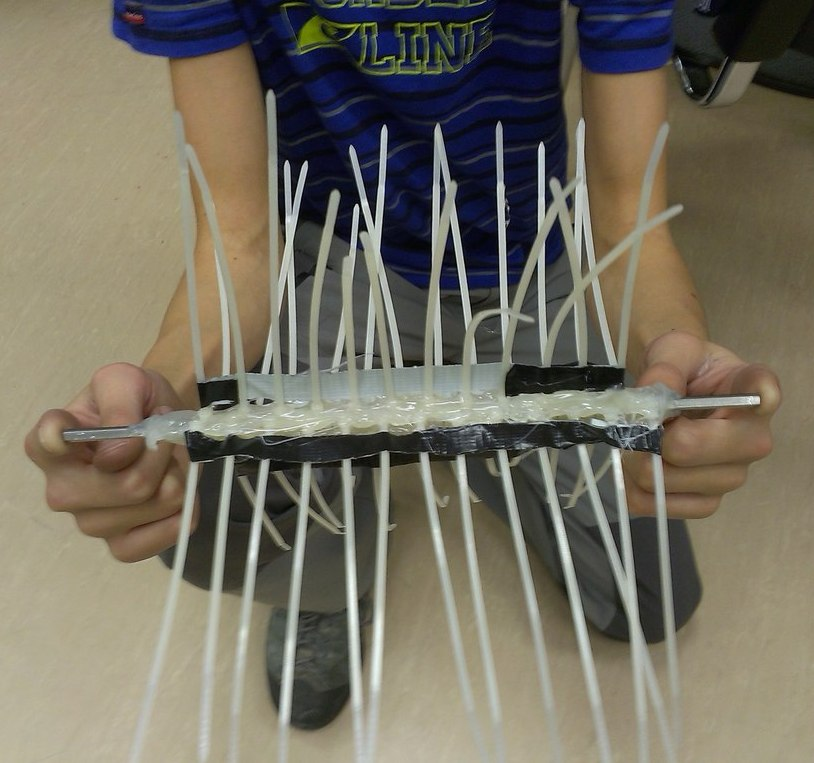
\includegraphics[scale=0.3]{days/18.10.14/images/01}}
      		\caption{Brush of gripper}
      	\end{minipage}
      	\hfill
      	\begin{minipage}[h]{0.47\linewidth}
      		\center{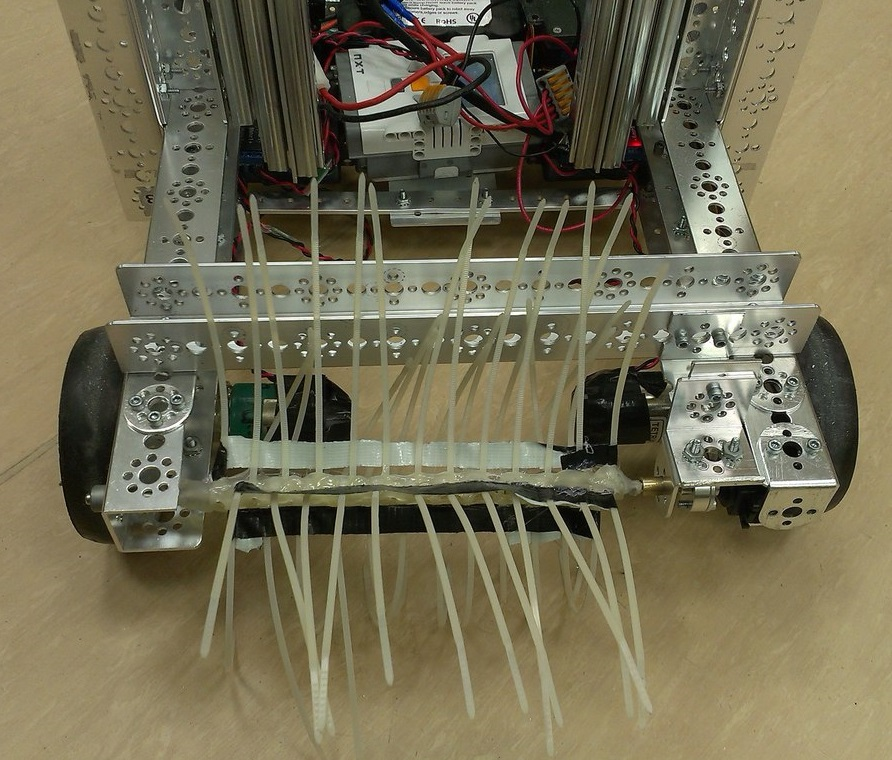
\includegraphics[scale=0.3]{days/18.10.14/images/02}}
      		\caption{The finished version of gripper for balls}
      	\end{minipage}
      \end{figure}
      
      \item Programme of control of gripper was changed. Now servo changes state (stop or running) by pressing the key. It allows to operator don't distracted to maintaining of gripper at working condition.   
      
      \item Were carried out tests of gripper with two balls from NXT set diametr 5cm. Robot can to capture balls at the open space and near the walls. Some inconvenience brought the fact that brush locates only at the center of robot and for capture of ball it need to aim to it. We planned to eliminate this disadvantage by installing on each side of the gripper beams located in a funnel (they hereinafter they will be referred to the slopes). It allows to balls to roll to scope capture.
      
      \item When was made the programme of control of servo it turned out that when servo is stopping it try to keep angle, what begins to rattle. This needs to be corrected.
      
      \item During testing it was turned out that robot stop to rattle when it turns around. It happened because a large part of it's mass was concentrated in the back part of robot so that the front wheels freely slipped.
      
      \item In addition the start tasks it was made mechanism of tipping bucket.
      
      \begin{figure}[H]
      	\begin{minipage}[h]{1\linewidth}
      		\center{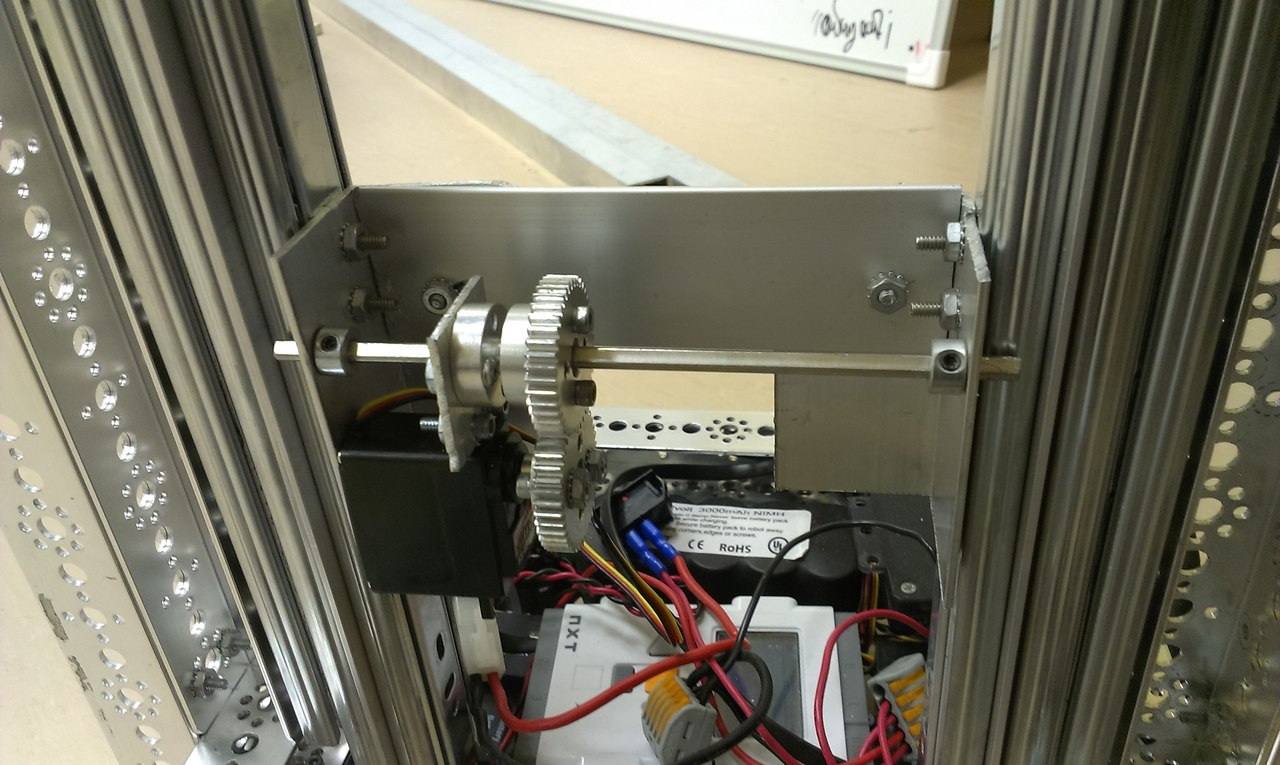
\includegraphics[scale=0.2]{days/18.10.14/images/03}}
      		\caption{Mechanism of tipping bucket}
      	\end{minipage}
      \end{figure}
      
    \end{enumerate}
    
	\item Results: 
	\begin{enumerate}
	  \item It was finished working on the gripper.
	  
      \item Was created more comfortable programme of control of the gripper.
      
    \end{enumerate}
    
	\item Tasks for the next congregations:
	\begin{enumerate}
	  \item Correct the problem with servo.
	  
	  \item Install the slopes.

    \end{enumerate}     
\end{enumerate}
\fillpage
